\documentclass[border=3pt,tikz]{standalone}
\usepackage{amsmath,amssymb,amsfonts}
\usepackage{tikz}
\usetikzlibrary{shapes,arrows.meta,positioning,calc,decorations.pathreplacing,decorations.markings,patterns,backgrounds,shadows,fit}

% Academic Color Palette
\definecolor{primaryblue}{RGB}{20, 45, 85}
\definecolor{accentblue}{RGB}{35, 85, 140}
\definecolor{safegreen}{RGB}{38, 115, 50}
\definecolor{safegreenbg}{RGB}{236, 246, 238}
\definecolor{safegreenborder}{RGB}{140, 200, 150}
\definecolor{dangerred}{RGB}{190, 35, 35}
\definecolor{dangerredbg}{RGB}{254, 237, 238}
\definecolor{dangerredborder}{RGB}{240, 160, 160}
\definecolor{warnorange}{RGB}{215, 100, 0}
\definecolor{warnyellowbg}{RGB}{255, 250, 235}
\definecolor{warnyellowborder}{RGB}{250, 210, 140}
\definecolor{tieorangebg}{RGB}{255, 242, 225}
\definecolor{tieorangeborder}{RGB}{250, 190, 120}
\definecolor{backupcolor}{RGB}{110, 35, 150}
\definecolor{backupbg}{RGB}{246, 238, 250}
\definecolor{panelbg}{RGB}{252, 253, 254}
\definecolor{panelborder}{RGB}{210, 218, 228}
\definecolor{darkslate}{RGB}{45, 55, 65}
\definecolor{midgray}{RGB}{125, 138, 150}

\begin{document}
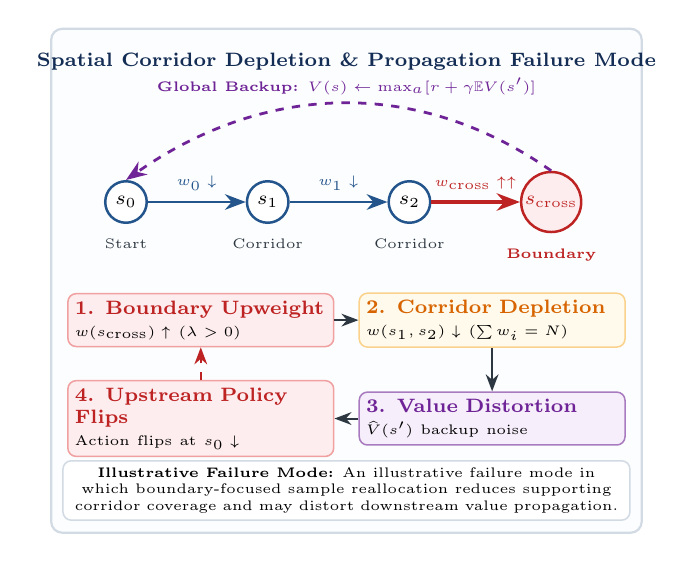
\begin{tikzpicture}[
    font=\small,
    >=Stealth,
    panel/.style={
        draw=panelborder,
        fill=panelbg,
        rounded corners=4pt,
        line width=0.8pt
    },
    boxcard/.style={
        rounded corners=3pt,
        line width=0.55pt,
        inner sep=2.8pt,
        font=\scriptsize
    },
    state/.style={
        circle,
        draw=accentblue,
        fill=white,
        line width=0.9pt,
        minimum size=15pt,
        inner sep=1pt,
        font=\scriptsize\bfseries
    }
]

\def\PW{7.5}
\def\PH{6.4}

\begin{scope}[shift={(0, 0)}]
    \draw[panel] (0,0) rectangle (\PW, \PH);
    \node[font=\bfseries\scriptsize, text=primaryblue, anchor=north] at (\PW/2, \PH-0.18) {Spatial Corridor Depletion \& Propagation Failure Mode};

    % Global Value Backup Annotation
    \node[font=\tiny\bfseries, text=backupcolor, anchor=north] at (\PW/2, \PH-0.5) {Global Backup: $V(s) \leftarrow \max_a [r + \gamma \mathbb{E} V(s')]$};

    % State Nodes
    \node[state] (N0) at (0.95, 4.2) {$s_0$};
    \node[state] (N1) at (2.75, 4.2) {$s_1$};
    \node[state] (N2) at (4.55, 4.2) {$s_2$};
    \node[state, draw=dangerred, fill=dangerredbg] (NC) at (6.35, 4.2) {\textcolor{dangerred}{$s_{\mathrm{cross}}$}};

    \node[font=\tiny, text=darkslate, below=2pt of N0] {Start};
    \node[font=\tiny, text=darkslate, below=2pt of N1] {Corridor};
    \node[font=\tiny, text=darkslate, below=2pt of N2] {Corridor};
    \node[font=\tiny\bfseries, text=dangerred, below=2pt of NC] {Boundary};

    % Bellman Backup Curved Arc
    \draw[->, backupcolor, dashed, line width=1.0pt] 
        (NC.north) to[out=145, in=35] (N0.north);

    % Forward Transition Arrows
    \draw[->, line width=1.0pt, accentblue] (N0) -- (N1) node[midway, above=0.5pt, font=\tiny] {$w_0 \downarrow$};
    \draw[->, line width=1.0pt, accentblue] (N1) -- (N2) node[midway, above=0.5pt, font=\tiny] {$w_1 \downarrow$};
    \draw[->, line width=1.2pt, dangerred] (N2) -- (NC) node[midway, above=0.5pt, font=\tiny, text=dangerred] {$w_{\mathrm{cross}} \uparrow\uparrow$};

    % Causal Degradation Pipeline
    \def\BW{3.35cm}
    
    \node[boxcard, fill=dangerredbg, draw=dangerredborder, minimum width=\BW, text width=3.2cm, align=left, inner sep=2.5pt] 
        (B1) at (1.9, 2.7) {
            \textbf{\textcolor{dangerred}{1. Boundary Upweight}}\\
            \tiny $w(s_{\mathrm{cross}}) \uparrow$ $(\lambda > 0)$
        };

    \node[boxcard, fill=warnyellowbg, draw=warnyellowborder, minimum width=\BW, text width=3.2cm, align=left, inner sep=2.5pt] 
        (B2) at (5.6, 2.7) {
            \textbf{\textcolor{warnorange}{2. Corridor Depletion}}\\
            \tiny $w(s_1, s_2) \downarrow$ $(\sum w_i = N)$
        };

    \node[boxcard, fill=backupbg, draw=backupcolor!60, minimum width=\BW, text width=3.2cm, align=left, inner sep=2.5pt] 
        (B3) at (5.6, 1.45) {
            \textbf{\textcolor{backupcolor}{3. Value Distortion}}\\
            \tiny $\widehat{V}(s')$ backup noise
        };

    \node[boxcard, fill=dangerredbg, draw=dangerredborder, minimum width=\BW, text width=3.2cm, align=left, inner sep=2.5pt] 
        (B4) at (1.9, 1.45) {
            \textbf{\textcolor{dangerred}{4. Upstream Policy Flips}}\\
            \tiny Action flips at $s_0 \downarrow$
        };

    % Sequence Arrows
    \draw[->, line width=0.7pt, darkslate] (B1.east) -- (B2.west);
    \draw[->, line width=0.7pt, darkslate] (B2.south) -- (B3.north);
    \draw[->, line width=0.7pt, darkslate] (B3.west) -- (B4.east);
    \draw[->, line width=0.7pt, dangerred, dashed] (B4.north) -- (B1.south);

    % Bottom Takeaway Box (Reviewer-Safe Wording)
    \node[boxcard, fill=white, draw=panelborder, anchor=south, minimum width=\PW cm - 0.3cm, inner sep=2.5pt] at (\PW/2, 0.15) {
        \parbox{6.9cm}{\centering \tiny \textbf{Illustrative Failure Mode:} An illustrative failure mode in which boundary-focused sample reallocation reduces supporting corridor coverage and may distort downstream value propagation.}
    };
\end{scope}

\end{tikzpicture}
\end{document}
